\section{Class Diagram}

%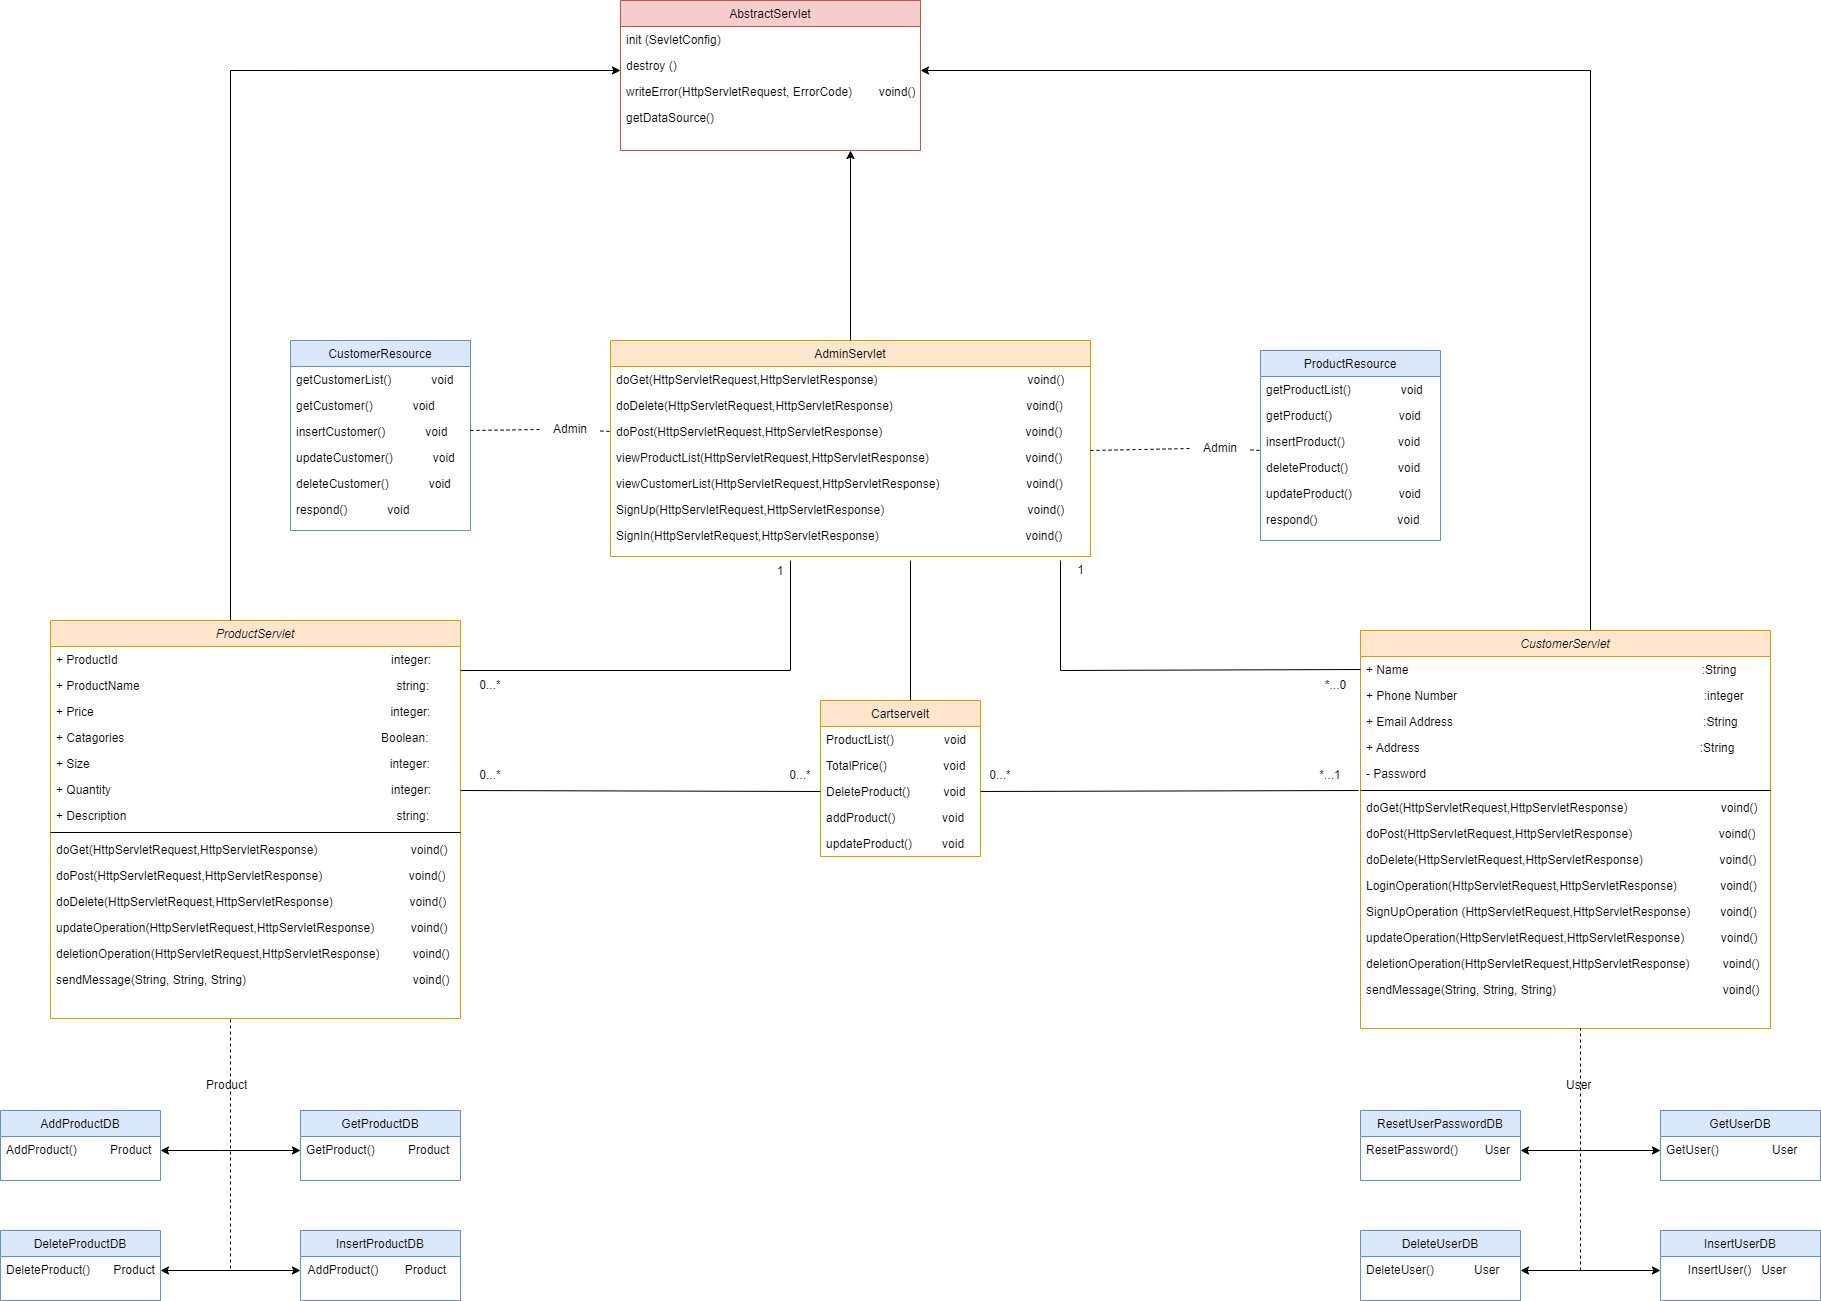
\includegraphics[width=\textwidth]{images/ClassDiagram.pdf}
\begin{figure}[h]
    \centering
    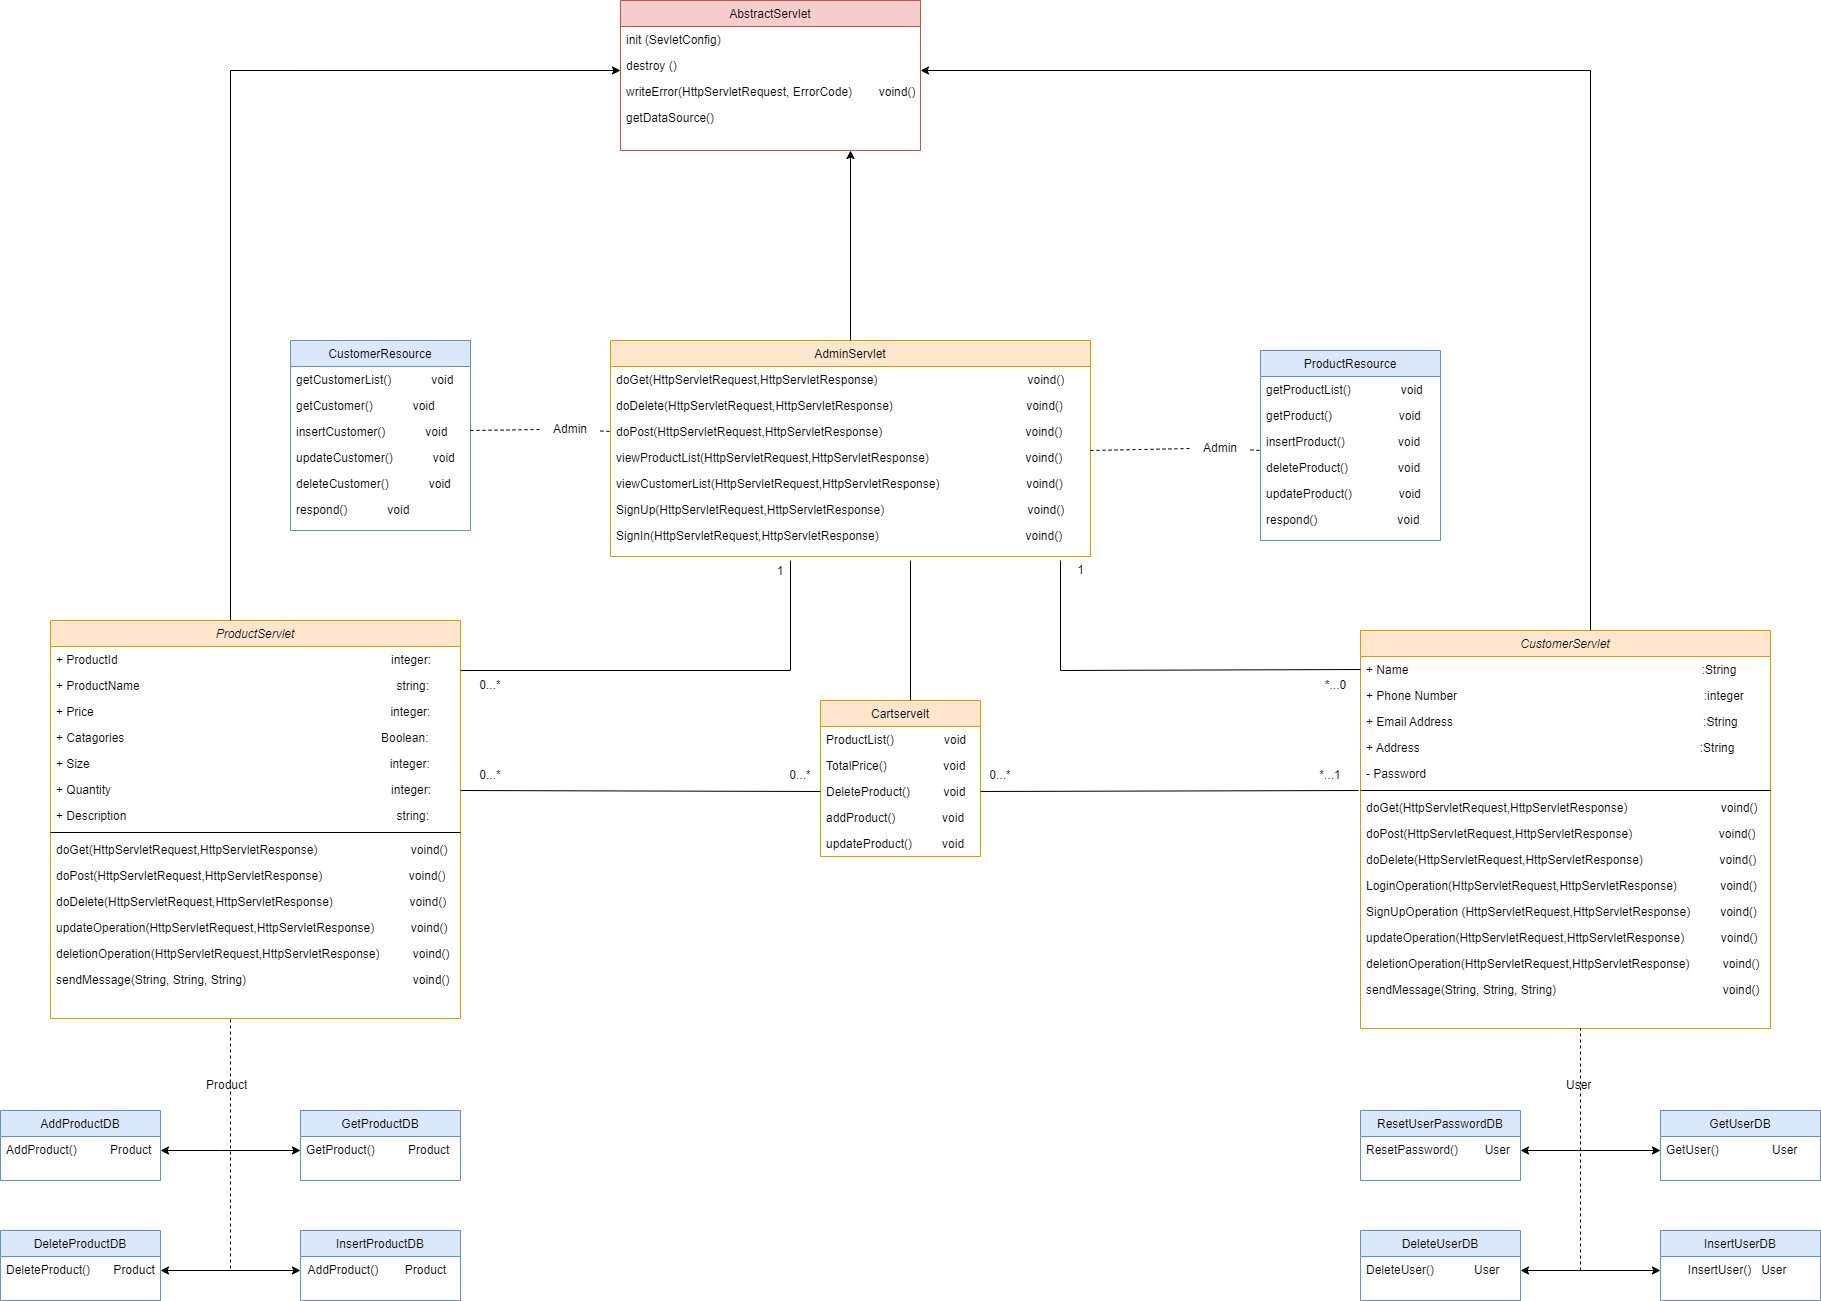
\includegraphics[width=1\textwidth]{images/ClassDiagram.png}
    \caption{Class Diagram}
    \label{FBPM}
\end{figure}

The class diagram contains (some of) the classes used to handle functionalities of the Admin, Customer and Cart in our system. AdminServlet, CustomerServlet and CartServlet are subclasses of the Java’s HttpServlet They are used to request functionalities accessible by the respective user and admin. The Connection Servlet is used to make connections to the database and consequently exchange data from it. The Authentication Servlet is used to authenticate each of the respective users. \newline
The CustomerResource and ProductResource are the subclasses of AdminServlet where the admin can control both pages and data. \newline
The Customer Class can register and can order a product without registration. Also, delete and add products to the cart list.
